\SourcePage{478}{481}
\chapter{Polyatomic Molecules}
\setcounter{section}{99}
\setcounter{figure}{40}
\section{Classification of Molecular Vibrations}

For polyatomic molecules, group theory first of all resolves the question of classifying their electronic terms, that is, the energy levels at a specified arrangement of the nuclei. They are classified according to the irreducible representations of the point symmetry group possessed by the nuclear configuration under consideration. It must, however, be stressed that the classification obtained in this way pertains precisely to this particular arrangement of the nuclei, since a displacement of the nuclei generally destroys the symmetry of the configuration. Usually the arrangement in question is the one corresponding to the equilibrium positions of the nuclei. In that case the classification retains a certain meaning also for small vibrations of the nuclei, but naturally loses its meaning when the vibrations cannot be regarded as small.

For a diatomic molecule we did not encounter this question, since its axial symmetry is of course preserved under any displacement of the nuclei. The situation is similar for triatomic molecules. Three nuclei always lie in one plane, which is a symmetry plane of the molecule. Consequently, the electronic terms of a triatomic molecule can always be classified with respect to this plane (by whether the wave functions are symmetric or antisymmetric under reflection in the plane).

There is an empirical rule for the normal electronic terms of polyatomic molecules: in the overwhelming majority of molecules, the wave function of the normal electronic state is totally symmetric (this rule was already mentioned for diatomic molecules in \S~78). In other words, it is invariant under every element of the molecular symmetry group, and thus belongs to the identity irreducible representation of the group.

Group-theoretical methods are especially important in the study of molecular vibrations (E.~Wigner, 1930). A purely classical treatment of the vibrations

\SourcePage{479}{482}
of a molecule as a system of a number of interacting particles (nuclei) must precede the quantum-mechanical study of this question.

As is known from mechanics (see I, \S~23, 24), a system of $N$ particles (not lying on one straight line) has $3N-6$ vibrational degrees of freedom; of the total $3N$ degrees of freedom, three correspond to translational and three to rotational motion of the system as a whole\footnote{If all the particles lie on one straight line, the number of vibrational degrees of freedom is $3N-5$ (rotation then has only two corresponding coordinates, so that rotation of a linear molecule about its own axis has no meaning).}. The energy of a system of particles executing small vibrations can be written as
\begin{equation}
 E=\frac12\sum_{i,k}m_{ik}\dot u_i\dot u_k+\frac12\sum_{i,k}k_{ik}u_i u_k. \tag{100.1}
\end{equation}
Here $m_{ik}$ and $k_{ik}$ are constant coefficients, while $u_i$ are components of the vectors giving the particles' displacements from their equilibrium positions (the indices $i$, $k$ enumerate both vector components and particles). By a suitable linear transformation of the quantities $u_i$, the coordinates corresponding to translation and rotation of the system can be eliminated from (100.1), and the vibrational coordinates can be chosen so that both quadratic forms in (100.1) become sums of squares. Normalizing these coordinates so that all coefficients in the kinetic-energy expression become unity, we obtain the vibrational energy in the form
\begin{equation}
 E=\frac12\sum_{i,\alpha}\dot Q_{\alpha i}^{2}+\frac12\sum_\alpha\omega_\alpha^2\sum_i Q_{\alpha i}^{2}. \tag{100.2}
\end{equation}

The vibrational coordinates $Q_{\alpha i}$ are called \emph{normal coordinates}; $\omega_\alpha$ are the frequencies of the corresponding independent vibrations. Several normal coordinates may have one and the same frequency (the frequency is then said to be \emph{multiple}); the index $\alpha$ of a normal coordinate specifies the frequency, while $i=1,2,\ldots,f_\alpha$ enumerates the coordinates belonging to that same frequency ($f_\alpha$ is the multiplicity of the frequency).

Expression (100.2) for the molecular energy must be invariant under symmetry transformations. This means that, under every transformation belonging to the molecule's point symmetry group, the normal coordinates $Q_{\alpha i}$, $i=1,2,\ldots,f_\alpha$ (for each fixed $\alpha$), transform linearly

\SourcePage{480}{483}
among themselves in such a way that the sum of squares $\sum_iQ_{\alpha i}^2$ remains unchanged.

In other words, the normal coordinates belonging to each given natural frequency of the molecule realize an irreducible representation of its symmetry group; the frequency multiplicity determines the dimension of the representation. Irreducibility follows from the same considerations given in \S~96 for solutions of the Schrödinger equation. Equality of frequencies corresponding to two different irreducible representations would be an extraordinarily unlikely coincidence. Here again a qualification is required: since physical normal coordinates are intrinsically real quantities, two complex-conjugate representations correspond to one natural frequency having twice the multiplicity.

These considerations make it possible to classify the natural vibrations of a molecule without solving the difficult problem of explicitly determining its normal coordinates. To do so, we must first find (by the method described below) the representation realized by all the vibrational coordinates together; we shall call it the complete \emph{vibrational representation}. This representation is reducible, and by decomposing it into irreducible parts we thereby determine the multiplicities of the natural frequencies and the symmetry properties of the corresponding vibrations. The same irreducible representation may occur several times in the complete representation; this means that there are several different frequencies of the same multiplicity whose vibrations have the same symmetry.

To find the complete vibrational representation, we use the fact that the characters of a representation are invariant under a linear transformation of the basis functions. Hence, in calculating them, we may use as basis functions not the normal coordinates but simply the components $u_i$ of the vectors giving the displacements of the nuclei from their equilibrium positions.

It is clear first of all that, when calculating the character of an element $G$ of the point group, only those nuclei which remain fixed (more precisely, whose equilibrium positions remain fixed) under the given symmetry transformation need be considered. Indeed, if under the rotation or reflection $G$ a nucleus 1 is moved to a new position previously occupied by another identical nucleus 2, the displacement of nucleus 1 is transformed under $G$ into the displacement of nucleus 2. In other words, the rows of the matrix $G_{ik}$ corresponding to this nucleus (that is, to its displacement $u_i$) will in any event contain no diagonal elements. The components of the displacement vector of a nucleus

\SourcePage{481}{484}
whose equilibrium position is unaffected by the operation $G$, on the other hand, transform only among themselves and can therefore be considered independently of the displacement vectors of the other nuclei.

Consider first a rotation $C(\varphi)$ through an angle $\varphi$ about a symmetry axis. Let $u_x$, $u_y$, $u_z$ be the components of the displacement vector of a nucleus whose equilibrium position lies on the axis itself and is therefore unaffected by the rotation. Under the rotation these components transform like those of any ordinary (polar) vector, according to the formulas (the $z$ axis coincides with the symmetry axis)
\[
 u_x'=u_x\cos\varphi+u_y\sin\varphi,\qquad
 u_y'=-u_x\sin\varphi+u_y\cos\varphi,\qquad
 u_z'=u_z.
\]
The character, that is, the sum of the diagonal elements of the transformation matrix, is $1+2\cos\varphi$. If a total of $N_C$ nuclei lie on this axis, the total character is
\begin{equation}
 N_C(1+2\cos\varphi). \tag{100.3}
\end{equation}
This character, however, corresponds to the transformation of all $3N$ displacements $u_i$; the part corresponding to the transformation of the translational displacement and the (small) rotation of the molecule as a whole must therefore be separated off. The translational displacement is specified by the displacement vector $\mathbf U$ of the molecular center of mass; its contribution to the character is consequently $1+2\cos\varphi$. The rotation of the molecule as a whole is specified by the rotation-angle vector $\delta\boldsymbol\Omega$\footnote{As is known, a small rotation angle can be regarded as a vector $\delta\boldsymbol\Omega$, whose magnitude equals the angle of rotation and whose direction is along the rotation axis in the sense fixed by the screw rule. A vector $\delta\boldsymbol\Omega$ defined in this way is evidently axial.}.

The vector $\delta\boldsymbol\Omega$ is axial; under rotations of the coordinate system, however, an axial vector behaves just like a polar vector. Thus $\delta\boldsymbol\Omega$ also has the character $1+2\cos\varphi$. In all, therefore, we must subtract $2(1+2\cos\varphi)$ from (100.3). We finally obtain the character $\chi(C)$ of the rotation $C(\varphi)$ in the complete vibrational representation:
\begin{equation}
 \chi(C)=(N_C-2)(1+2\cos\varphi). \tag{100.4}
\end{equation}
The character of the identity element $E$ is evidently just the total number of vibrational degrees of freedom: $\chi(E)=3N-6$ (this also follows from (100.4) with $N_C=N$, $\varphi=0$).

\SourcePage{482}{485}
In the same way we calculate the character of the rotation--reflection transformation $S(\varphi)$ (a rotation through $\varphi$ about the $z$ axis followed by reflection in the $xy$ plane). Under this transformation a vector changes according to
\[
 u_x'=u_x\cos\varphi+u_y\sin\varphi,\qquad
 u_y'=-u_x\sin\varphi+u_y\cos\varphi,\qquad
 u_z'=-u_z,
\]
which has the character $(-1+2\cos\varphi)$. The character of the representation realized by all $3N$ displacements $u_i$ is therefore
\begin{equation}
 N_S(-1+2\cos\varphi), \tag{100.5}
\end{equation}
where $N_S$ is the number of nuclei unaffected by the operation $S(\varphi)$ (this number can evidently be either zero or one). The displacement vector $\mathbf L$ of the center of mass has the character $(-1+2\cos\varphi)$. As for $\delta\boldsymbol\Omega$, being an axial vector it is unchanged by inversion of the coordinate system; on the other hand, the rotation--reflection transformation $S(\varphi)$ can be written
\[
 S(\varphi)=C(\varphi)\sigma_h=C(\varphi)C_2I=C(\pi+\varphi)I,
\]
that is, as a rotation through $\pi+\varphi$ followed by inversion. Consequently, the character of $S(\varphi)$ acting on $\delta\boldsymbol\Omega$ is equal to the character of $C(\pi+\varphi)$ acting on an ordinary vector, namely $1+2\cos(\pi+\varphi)=1-2\cos\varphi$. The sum $(-1+2\cos\varphi)+(1-2\cos\varphi)=0$, and we thus reach the result that expression (100.5) itself is the required character $\chi(S)$ of the rotation--reflection transformation $S(\varphi)$ in the complete vibrational representation:
\begin{equation}
 \chi(S)=N_S(-1+2\cos\varphi). \tag{100.6}
\end{equation}
In particular, the character of reflection in a plane ($\varphi=0$) is $\chi(\sigma)=N_\sigma$, while the character of inversion ($\varphi=\pi$) is $\chi(I)=-3N_I$.

Once the characters $\chi$ of the complete vibrational representation have been found, it remains only to decompose it into irreducible representations. This is done from formula (94.16), using the character tables given in \S~95 (see the problems to this section).

Group theory is not needed to classify the vibrations of a linear molecule. The total number of vibrational degrees of freedom is $3N-5$. Among the vibrations one must distinguish those in which the atoms remain on one straight line from

\SourcePage{483}{486}
those in which they do not\footnote{If the molecule is symmetric about its midpoint, there is one further characteristic of the vibrations; see problem 10 to this section.}. The number of degrees of freedom for the motion of $N$ particles along a line is $N$; one of them corresponds to translational motion of the molecule as a whole. Hence the number of normal coordinates for vibrations that leave the atoms on a straight line is $N-1$; in general, these correspond to $N-1$ different natural frequencies. The remaining $(3N-5)-(N-1)=2N-4$ normal coordinates belong to vibrations that destroy the linearity of the molecule; they correspond to $N-2$ different double frequencies (each frequency has two normal coordinates, describing identical vibrations in two mutually perpendicular planes)\footnote{In the notation for the irreducible representations of the group $C_{\infty v}$ (\S~98), there are $N-1$ vibrations of type $A_1$ and $N-2$ vibrations of type $E_1$.}.

\subsection*{Problems}

\ProblemHeading{1.} Classify the normal vibrations of the $\mathrm{NH_3}$ molecule (a regular pyramid with the N atom at its apex and the H atoms at the corners of its base; Fig.~41).

\SolutionHeading The molecular point symmetry group is $C_{3v}$. Rotations about the threefold axis leave only one atom (N) fixed, while reflections in the planes leave two atoms fixed (N and one H). From formulas (100.4), (100.6), the characters of the complete vibrational representation are
\[
\begin{array}{c|ccc} &E&2C_3&3\sigma_v\\\hline &6&0&2\end{array}
\]
\begin{figure}[ht]
\centering
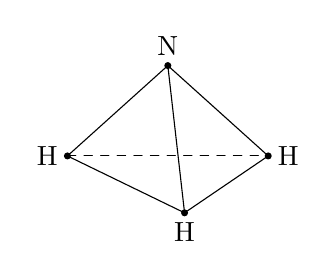
\begin{tikzpicture}[scale=.85,line cap=round]
\coordinate (N) at (0,1.35); \coordinate (L) at (-1.5,0); \coordinate (R) at (1.5,0); \coordinate (B) at (.25,-.85);
\draw (N)--(L)--(B)--(R)--cycle; \draw[dashed] (L)--(R); \draw (N)--(B);
\foreach \p in {N,L,R,B}\fill (\p) circle (1.5pt);
\node[above] at (N){N}; \node[left] at (L){H}; \node[right] at (R){H}; \node[below] at (B){H};
\end{tikzpicture}
\caption{}
\end{figure}
Decomposing this representation into irreducible parts, we find that it contains the representation $A_1$ twice and $E$ twice. There are therefore two simple frequencies corresponding to vibrations of type $A_1$, which preserve the full symmetry of the molecule (the so-called totally symmetric vibrations), and two double frequencies corresponding to normal coordinates that transform into one another according to the representation $E$.

\ProblemHeading{2.} Do the same for the $\mathrm{H_2O}$ molecule (Fig.~42).

\begin{figure}[ht]
\centering
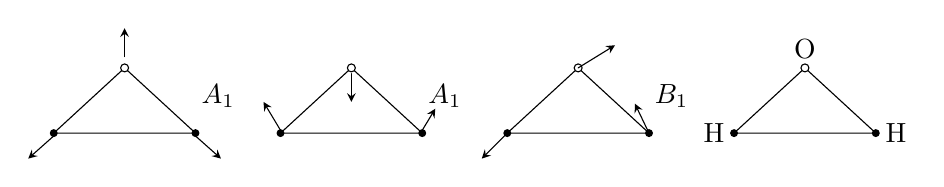
\begin{tikzpicture}[>=stealth,scale=.72,line cap=round]
\foreach \x/\lab in {0/$A_1$,4/$A_1$,8/$B_1$}{
 \coordinate (o) at (\x,1.15); \coordinate (l) at (\x-1.25,0); \coordinate (r) at (\x+1.25,0);
 \draw (l)--(o)--(r) (l)--(r); \fill (l) circle(2pt) (r) circle(2pt); \draw[fill=white] (o) circle(2pt); \node at (\x+1.65,.65){\lab};}
\draw[->] (0,1.35)--(0,1.85); \draw[->] (-1.25,-.05)--(-1.7,-.45); \draw[->] (1.25,-.05)--(1.7,-.45);
\draw[->] (4,1.05)--(4,.55); \draw[->] (2.75,.05)--(2.45,.55); \draw[->] (5.25,.05)--(5.48,.43);
\draw[->] (8,1.15)--(8.65,1.55); \draw[->] (6.75,0)--(6.3,-.45); \draw[->] (9.25,0)--(9.0,.52);
\coordinate (O) at (12,1.15); \coordinate (H1) at (10.75,0); \coordinate (H2) at (13.25,0); \draw (H1)--(O)--(H2) (H1)--(H2); \fill (H1) circle(2pt) (H2) circle(2pt); \draw[fill=white] (O) circle(2pt); \node[above] at (O){O}; \node[left] at (H1){H}; \node[right] at (H2){H};
\end{tikzpicture}
\caption{}
\end{figure}

\SolutionHeading The symmetry group is $C_{2v}$. The transformation $C_2$ leaves the O atom fixed, the transformation $\sigma_v$ (reflection in the molecular plane) leaves all three atoms fixed, and the reflection $\sigma_v'$ leaves only the O atom fixed. The characters of the complete vibrational representation are
\[
\begin{array}{c|cccc}&E&C_2&\sigma_v&\sigma_v'\\\hline&3&1&3&1\end{array}
\]

\SourcePage{484}{487}
This representation decomposes into the irreducible representations $2A_1$, $1B_1$: there are two totally symmetric vibrations and one whose symmetry is specified by the representation $B_1$; all the frequencies are simple (Fig.~42 shows the corresponding normal vibrations).

\ProblemHeading{3.} Do the same for the $\mathrm{CH_3Cl}$ molecule (Fig.~43\textit{a}).

\SolutionHeading The molecular symmetry group is $C_{3v}$. The same method shows that there are three totally symmetric vibrations $A_1$ and three double vibrations of type $E$.

\begin{figure}[p]
\centering
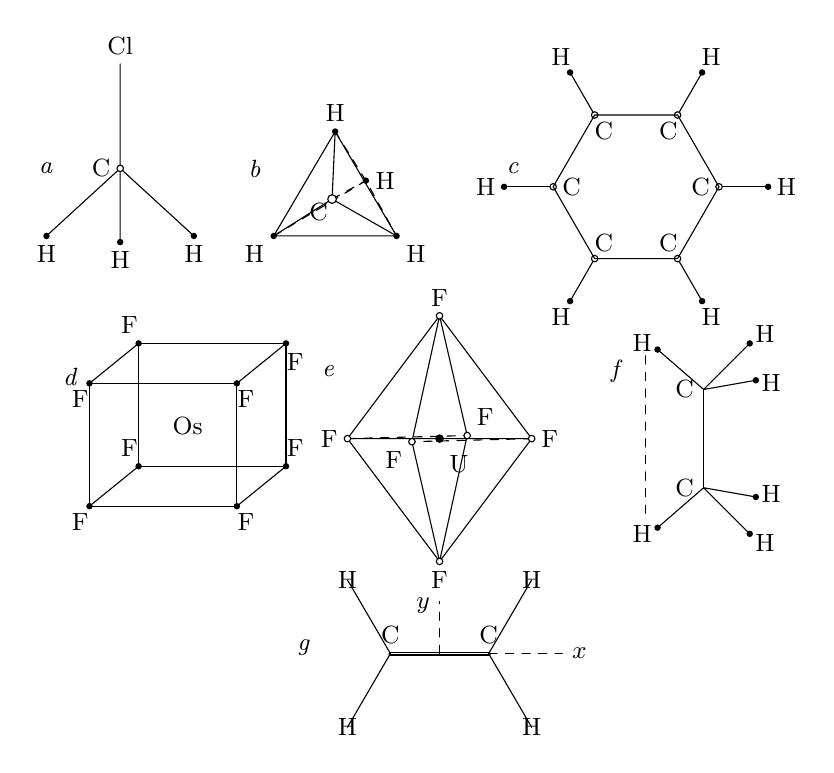
\begin{tikzpicture}[scale=.78,line cap=round,font=\small]
% a CH3Cl
\begin{scope}[shift={(-5.2,4.3)}]\node at (-1.2,.3){\textit{a}}; \coordinate(C)at(0,.3);\coordinate(Cl)at(0,2);\draw(C)--(Cl) (C)--(-1.2,-.8) (C)--(0,-.9) (C)--(1.2,-.8);\draw[fill=white](C)circle(1.5pt);\node[left]at(C){C};\node[above]at(Cl){Cl};\foreach\p in {(-1.2,-.8),(0,-.9),(1.2,-.8)}\fill\p circle(1.5pt);\node[below]at(-1.2,-.8){H};\node[below]at(0,-.9){H};\node[below]at(1.2,-.8){H};\end{scope}
% b CH4 tetrahedron
\begin{scope}[shift={(-1.7,4.3)}]\node at(-1.3,.3){\textit{b}};\coordinate(T)at(0,.9);\coordinate(L)at(-1,-.8);\coordinate(R)at(1,-.8);\coordinate(M)at(.5,.1);\coordinate(C)at(-.05,-.2);\draw(T)--(L)--(R)--cycle;\draw[dashed](L)--(M)--(R) (T)--(M);\draw(C)--(T) (C)--(L) (C)--(R);\draw[dashed](C)--(M);\draw[fill=white](C)circle(2pt);\fill(T)circle(1.5pt)(L)circle(1.5pt)(R)circle(1.5pt)(M)circle(1.5pt);\node[above]at(T){H};\node[below left]at(L){H};\node[below right]at(R){H};\node[right]at(M){H};\node[below left=-2pt]at(C){C};\end{scope}
% c benzene
\begin{scope}[shift={(3.2,4.3)}]\node at(-2,.3){\textit{c}};\foreach\i in{0,...,5}{\coordinate(C\i)at({60*\i}:1.35);\coordinate(H\i)at({60*\i}:2.15);\draw(C\i)--(H\i);\draw[fill=white](C\i)circle(1.5pt);\fill(H\i)circle(1.5pt);\node at({60*\i}:1.05){C};\node at({60*\i}:2.45){H};}\draw(C0)--(C1)--(C2)--(C3)--(C4)--(C5)--cycle;\end{scope}
% d cube OsF8
\begin{scope}[shift={(-4.5,.1)}]\node at(-1.5,1.1){\textit{d}};\draw(-1.2,-1)--(1.2,-1)--(1.2,1)--(-1.2,1)--cycle;\draw(-.4,-.35)--(2,-.35)--(2,1.65)--(-.4,1.65)--cycle;\draw(-1.2,-1)--(-.4,-.35) (1.2,-1)--(2,-.35) (1.2,1)--(2,1.65) (-1.2,1)--(-.4,1.65);\foreach\p in{(-1.2,-1),(1.2,-1),(1.2,1),(-1.2,1),(-.4,-.35),(2,-.35),(2,1.65),(-.4,1.65)}\fill\p circle(1.5pt);\node at(.4,.3){Os};\foreach\p in{(-1.35,-1.25),(1.35,-1.25),(1.35,.75),(-1.35,.75),(-.55,-.05),(2.15,-.05),(2.15,1.35),(-.55,1.95)}\node at\p{F};\end{scope}
% e UF6 octahedron
\begin{scope}[shift={(0,.2)}]\node at(-1.8,1.1){\textit{e}};\coordinate(T)at(0,2);\coordinate(B)at(0,-2);\coordinate(L)at(-1.5,0);\coordinate(R)at(1.5,0);\coordinate(F)at(-.45,-.05);\coordinate(K)at(.45,.05);\draw(T)--(L)--(B)--(R)--cycle (T)--(F)--(B) (T)--(K)--(B) (L)--(R);\draw[dashed](L)--(K) (R)--(F);\fill(0,0)circle(2pt);\node[below right]at(0,-.12){U};\foreach\p in{T,B,L,R,F,K}\draw[fill=white](\p)circle(1.5pt);\node[above]at(T){F};\node[below]at(B){F};\node[left]at(L){F};\node[right]at(R){F};\node[below left]at(F){F};\node[above right]at(K){F};\end{scope}
% f ethane
\begin{scope}[shift={(4.3,.2)}]\node at(-1.4,1.1){\textit{f}};\coordinate(Ct)at(0,.8);\coordinate(Cb)at(0,-.8);\draw(Ct)--(Cb);\node[left]at(Ct){C};\node[left]at(Cb){C};\foreach\p in{(-.75,1.45),(.75,1.55),(.85,.95),(-.75,-1.45),(.75,-1.55),(.85,-.95)}\fill\p circle(1.5pt);\draw(Ct)--(-.75,1.45) (Ct)--(.75,1.55) (Ct)--(.85,.95) (Cb)--(-.75,-1.45) (Cb)--(.75,-1.55) (Cb)--(.85,-.95);\foreach\p in{(-1,1.55),(1,1.7),(1.1,.9),(-1,-1.55),(1,-1.7),(1.1,-.9)}\node at\p{H};\draw[dashed](-.95,1.35)--(-.95,-1.35);\end{scope}
% g ethylene
\begin{scope}[shift={(0,-3.3)}]\node at(-2.2,.1){\textit{g}};\coordinate(CL)at(-.8,0);\coordinate(CR)at(.8,0);\draw[double](CL)--(CR);\node[above]at(CL){C};\node[above]at(CR){C};\draw(CL)--(-1.5,1.2) (CL)--(-1.5,-1.2) (CR)--(1.5,1.2) (CR)--(1.5,-1.2);\foreach\p in{(-1.5,1.2),(-1.5,-1.2),(1.5,1.2),(1.5,-1.2)}\node at\p{H};\draw[dashed](0,0)--(0,.85) (.8,0)--(2,0);\node[left]at(0,.78){$y$};\node[right]at(2,0){$x$};\end{scope}
\end{tikzpicture}
\caption{}
\end{figure}
\clearpage

\ProblemHeading{4.} Do the same for the $\mathrm{CH_4}$ molecule (the C atom is at the center and the H atoms are at the vertices of a tetrahedron; Fig.~43\textit{b}).

\SolutionHeading The molecular symmetry is $T_d$. The vibrations are $1A_1$, $1E$, $2F_2$.

\ProblemHeading{5.} Do the same for the $\mathrm{C_6H_6}$ molecule (Fig.~43\textit{c}).

\SolutionHeading The molecular symmetry is $D_{6h}$. The vibrations are
\[
2A_{1g},1A_{2g},1A_{2u},1B_{1g},1B_{1u},1B_{2g},3B_{2u},1E_{1g},3E_{1u},4E_{2g},2E_{2u}.
\]

\ProblemHeading{6.} Do the same for the $\mathrm{OsF_8}$ molecule (the Os atom is at the center and the F atoms are at the vertices of a cube; Fig.~43\textit{d}).

\SolutionHeading The molecular symmetry is $O_h$. The vibrations are
\[
1A_{1g},1A_{2u},1E_g,1E_u,2F_{1u},2F_{2g},2F_{2u}.
\]

\ProblemHeading{7.} Do the same for the $\mathrm{UF_6}$ molecule (the U atom is at the center and the F atoms are at the vertices of an octahedron; Fig.~43\textit{e}).

\SourcePage{485}{488}
\SolutionHeading The molecular symmetry is $O_h$. The vibrations are
\[
1A_{1g},1E_g,2F_{1u},1F_{2g},1F_{2u}.
\]

\ProblemHeading{8.} Do the same for the $\mathrm{C_2H_6}$ molecule (Fig.~43\textit{f}).

\SolutionHeading The molecular symmetry is $D_{3d}$. The vibrations are
\[
3A_{1g},1A_{1u},2A_{2u},3E_g,3E_u.
\]

\ProblemHeading{9.} Do the same for the $\mathrm{C_2H_4}$ molecule (Fig.~43\textit{g}; all the atoms lie in one plane).

\SolutionHeading The molecular symmetry is $D_{2h}$. The vibrations are
\[
3A_{1g},1A_{1u},2B_{1g},1B_{1u},2B_{3u},1B_{2g},2B_{2u}
\]
(the coordinate axes are chosen as shown in the figure).

\ProblemHeading{10.} Do the same for a linear molecule of $N$ atoms symmetric about its midpoint.

\SolutionHeading To the classification of the vibrations of a linear molecule considered in the text, one must add classification by their behavior under inversion in the center. The cases of even and odd $N$ must be distinguished.

If $N$ is even ($N=2p$), there is no atom at the midpoint of the molecule. Give the $p$ atoms in one half of the molecule independent displacements along the line, and the other $p$ atoms equal and opposite displacements. We then find that $p$ of the vibrations which leave the atoms on the line are symmetric about the center, while the remaining $(2p-1)-p=p-1$ vibrations of this type are antisymmetric about the center. Next, the $p$ atoms have $2p$ degrees of freedom for motions in which the atoms are not constrained to the line. Giving symmetrically situated atoms equal and opposite displacements would produce $2p$ symmetric vibrations; from this number, however, two corresponding to rotation of the molecule must be subtracted. There are therefore $p-1$ double frequencies for vibrations that carry the atoms off the line and are symmetric about the center, and the same number $((2p-2)-(p-1)=p-1)$ that are antisymmetric. In the notation for the irreducible representations of the group $D_{\infty h}$ (see the end of \S~98), there are $p$ vibrations of type $A_{1g}$ and $(p-1)$ vibrations of each of the types $A_{1u}$, $E_{1g}$, $E_{1u}$.

If $N$ is odd ($N=2p+1$), analogous reasoning shows that there are $p$ vibrations of each of the types $A_{1g}$, $A_{1u}$, $E_{1u}$, and $(p-1)$ vibrations of type $E_{1g}$.
